\question %8
\emph{Implémentez sous MATLAB ce modèle linéaire continu,
et calculez la solution correspondant aux données fournies sur icampus.
Commentez l'allure de la solution obtenue, et comparez à la solution du modèle
simplifié. Commentez également l'intégralité des variables de la solution ;
celle-ci présente-t-elle un aspect problématique ?}

\begin{figure}[H]
  \begin{center}
    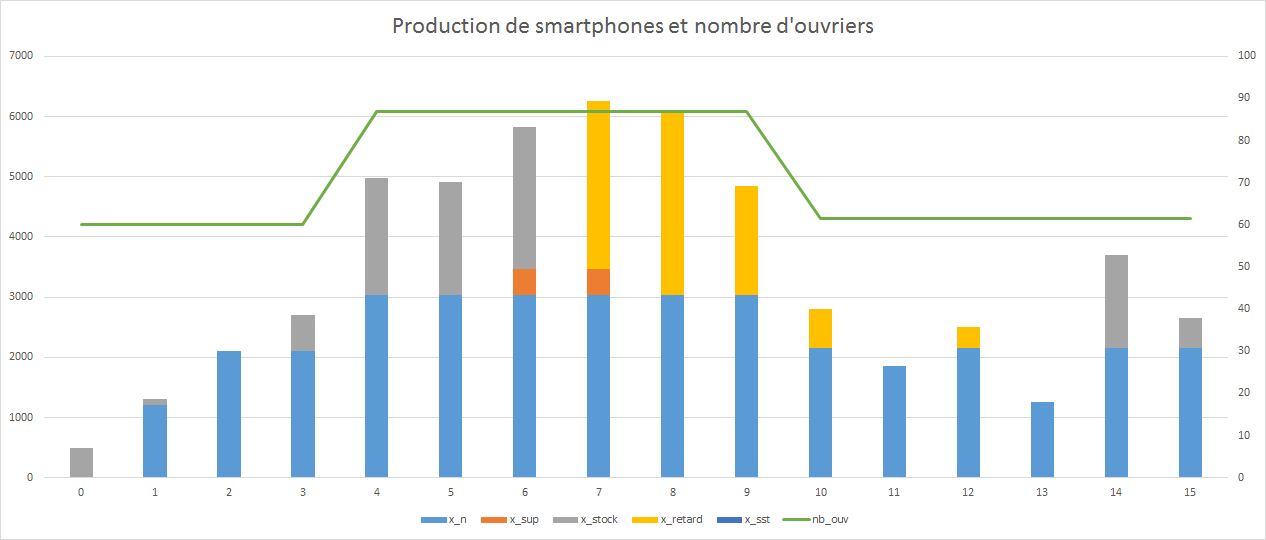
\includegraphics[scale = 0.75]{img/grapheProductionOuvNonInt.png}
	  \caption{Répartition du moyen de production des smartphones en fonction des semaines et évolution du nombre d'ouvriers dans le cas non entier.}
	  \label{fig:grapheProductionOuvNonInt}
  \end{center}
\end{figure}

Les résultats de cette nouvelle implémentation sont présentés à la figure \ref{fig:grapheProductionOuvNonInt}. Les résultats obtenus ne sont plus entiers car le problème ne peut plus être reformulé comme un problème de flot. Ceci est problématique car il serait impossible de réaliser cette production exacte en pratique. Pour les applications, il est plus intéressant de chercher la solution otimale entière. C'est pourquoi nous commenterons l'allure de la solution à la question 9 où nous avons résolu le problème en variables entières. Néanmoins, nous pouvons déjà faire deux remarques à ce stade :
\begin{itemize}
\item Le coût est ici de 3.755.214 unités. En comparaison, le coût obtenu par résolution en variables entières est de 3.755.300 unités. Il y a donc une différence de coût, certes très faible. La nouvelle contrainte appliquée au système, celle de résoudre en variables entières, nous fait perdre en efficacité. 
\item Les résultats du modèle en variables continues sont très semblables à ceux du modèle en variables entières, présentés à la figure \ref{fig:grapheProductionOuv}. La seule différence notable est l'utilisation de retard à la place d'ouvriers payés au salaire des heures supplémentaires lors de la huitième semaine, probablement due à la faible différence de coût entre les deux possibilités.
\end{itemize}

Notre fonction MATLAB relative à cette question est \texttt{question8.m}. Nous vous invitons à taper \texttt{help question8} en ligne de commande afin de savoir comment interagir avec celle-ci.